% !TEX root = ../main.tex


\section{Introductory Remarks}




%decentralized exchanges allow the market participants to be fully authoritative over their assets using their private keys. 
%One issue with decentralized 
%
%Cryptocurrency trading on centralized exchanges has been shown to be vulnerable to cybersecurity hacking and internal frauds over the years, with the most infamous hacks being Mt. Gox and Coincheck. In addition, trading on centralized exchanges is not compatible with DeFi applications since it is technically infeasible to bridge between decentralized applications and centralized servers without compromising the trust model.







% = = = = = = = = = = = = = = = = = = = = = = = = = = = = = = = = = = = = = = = = = =

\section{Order Books}

Order books are data structures that maintain lists of bid and ask orders for various assets (\eg currencies, stocks, bonds \etc) in specific markets. The most common version of order books is what we call a \textit{double auction}, where market participants submit their bid and ask orders and the market clearing price will be calculated as the average between the best bid and best ask prices. Order books often sort the orders based on their price and submission time (this order allocation technique is called price-time priority)~\cite{preis2011price}, where orders are prioritized from highest price to lowest and given any two orders with the same price, they will be sorted based on their submission timestamps.

\par

Looking more closely, order books are rather electronic ledgers that get updated over time. Given the definition of the Etehreum blockchain (\ie a distributed ledger), the idea of implementing an order book in the form of a smart contract will seemingly resolve the existing issues with centralized exchanges. However, this design is not feasible due to some crucial challenges that exist within blockchains:

\begin{itemize}

\item \textbf{Speed.}

\item \textbf{Front-running and Censorship.}

\item \textbf{Enforcing Time.}

\end{itemize}


% = = = = = = = = = = = = = = = = = = = = = = = = = = = = = = = = = = = = = = = = = =






% = = = = = = = = = = = =Notes Discussed in Meetings = = = = = = = = = = = = =  %

% Our two competitors are Uinswap and Loopring (that uses ZK roll ups):
% 	1- Uniswap: we can argue that in traditional markets we have various traditional exchanges. Each of these exchanges have different trading rules and designs which work for different traders.
%	2- Loopring:
%		2-1: Barrier to entry: In order for a trader to trade specific ERC20 on Loopring, Loopring has to agree to support that token. It might not be difficult and they probably approve the token as long as it is standard compliant.
%		2-2: ZK proofs are quick and cheap to verify but they are expensive and time consuming to generate: (1) now they are generating these proofs for free but later they charge traders for doing that. (2) Looping does not probably generate these proofs per every block so the settlement and 				clearing is not happening per block. So we have faster clearing and settlement as we clear everything per block. 
% 		2-3: Loopring is non-custodial, meaning that the money moves only when the proofs come, so there is a latency in transferring funds to the traders.


% The heap with dynamic array can do 26 pairs of matches at worst case matching whereas Linkedliat does 90 pairs. So if we want to cap the orders over 4 PQs, we’re basically increasing the heap size which makes match more expensive for nothing (every time a match happens and the root is deleted the whole heap is reheapified)

% There will be no ties as we use 2 counters for buy and sell orders. These counters are concatenated them with the price. So we somehow enforce time priority




% = = = = = = = = = = = =Clearing Mappings = = = = = = = = = = = = =  %
\section{Clearing Mappings}

To facilitate a safe exchange among buyers and sellers, we implement the CallMarket smart contract in the form of a \textit{collateralized}; for market participants to be able to send bid and/or ask orders, they have to first supply assets (depending on what asset they aim to trade) as collaterals  by calling any of the  \texttt{DepositToken()} or \texttt{DepositEther()} methods. The collateralized CallMarket acts as a payment guarantees and market participants cannot default on payment or delivery of their assets.

To maintain the collateral balance of each market participant, we use two Solidity type one-to-one mapping that map Ethereum addresses to 256 bits unsigned integers; \texttt{TotalBalance} and \texttt{UnavailableBalance}. Once market closes and orders are matched, the \texttt{UnavailableBalance} needs to be cleared. However, since it is not possible to delete the entire mapping without knowing the keys~\footnote{https://solidity.readthedocs.io/en/v0.5.12/security-considerations.html}, clearing the \texttt{UnavailableBalance} mapping remains a challenging issue to solve . Here we provide a landscape of solutions for that.
%only individual keys and what they map to can be deleted.

\begin{enumerate}

\item \textbf{Creating a New Mapping Every Time the Market Opens.} Instead of clearing the \texttt{UnavailableBalance} of traders at the end of a matching process, we could create a new mapping every time the market opens. Note that using this solution, traders can only claim their funds (using the \texttt{ClaimEther()} and/or \texttt{ClaimToken} methods) only when the market is in state \texttt{Closed}. 

\item \textbf{Creating Custom Keys for the Mapping.} We can create custom keys for the mapping by defining a counter as a global variable inside the CallMarket smart contract. This counter is incremented at the end of the matching process. So instead of clearing the mapping, we only use another portion of it every time the market opens.

\item \textbf{Storing the Mapping in a Data-Contract.} Another design proposal is to create a smart contract every time the market opens, this data contract only stores the \texttt{UnavailableBalance} mapping and will be killed at the end of the matching process.

\item \textbf{Storing the Mapping keys in an Array.} We can create an array that stores the traders' addresses (\ie the mapping keys). Knowing the keys enable us to iterate over the mapping and delete individual keys and what they map to at the end of the matching process. This is a gas-costly design pattern and would cause a high probability of exceeding the gas limitation inside the \texttt{Match()} function.



\end{enumerate}

 %Deleting the unavailable mapping remains a challenging issue to solve (have a little section in the paper to discuss our different solutions for it). 
%	1- we can just create a new mapping everytime the market opens and have a modifier for the claim functions so that they could be called only when the market is closed. 
%	2- we can have custom keys for the mapping (like a counter we define as a global variable and increment it at the end of the match function). So everytime the new market starts, we just use another portion of the mapping.
%	3- we can have another smart contract which only stores the mapping and just delete that after the close function. 


% = = = = = = = = = = = = = = = = = = = = = = = = = = = = = = = = = %




% = = = = = = = = = = = =Who pays for the close function? = = = = = = = = = = = = =  %

\section{Who Pays the Cost for the \texttt{CloseMarket()} Function?}

Ethereum contracts can only run when a function is called. So if no one calls the \texttt{CloseMarket()} function at the end of the trading period, this function cannot self-execute to modify itself. In addition, upon closing the market the \texttt{Match()} function will be executed which consumes a significant amounts of gas, and the person who closes the market must have enough incentives to do so. We think it is useful to explore the landscape of possible designs for closing the market. 

\begin{enumerate}

\item \textbf {Using the Meta Transactions.} Meta transactions enable users to execute Ethereum functions without paying the gas. Rather than spending gas, users sign their intended action using their private keys and broadcast it to the network with no cost. A third party process (\textit{a relayer}) then crafts the actual transaction on user's behalf, sends the transaction to the Ethereum blockchain, and charges the base contract with the associated fees (see Figure~\ref{fig:meta_tx}). The required gas to pay for the \texttt{Match()} function could be collected as fees. So market participants are charged with certain amounts of fees every time they submit an order, these fees are accumulated in the CallMarket contract and will be used to pay for executing the \texttt{CloseMarket()} function.

% = = = = = = = = = = = =meta_tx Figure = = = = = = = = = = = = =  %

\begin{figure}[htb!p]
\centering
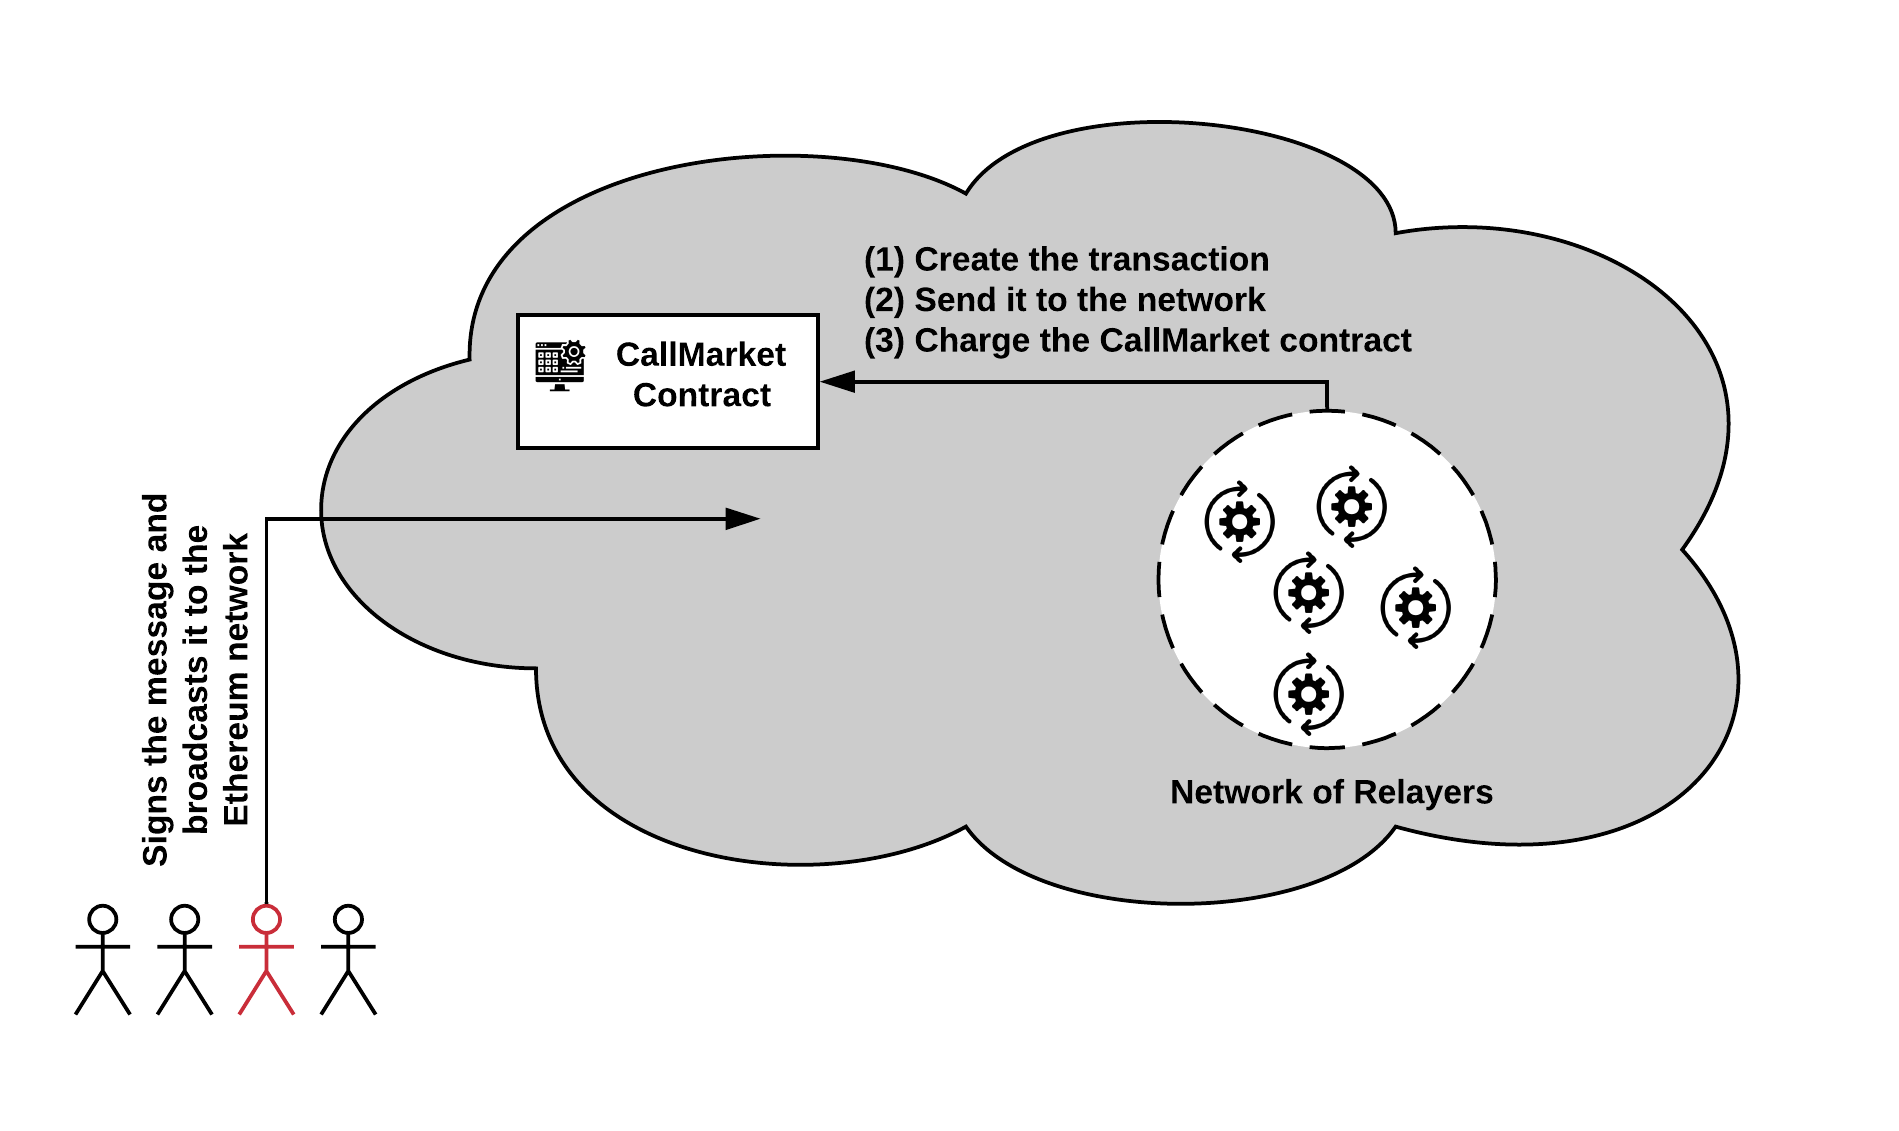
\includegraphics[width=0.8\textwidth]{fig/meta_tx.png}
\caption{\footnotesize{}  \label{fig:meta_tx}}
\end{figure}

% = = = = = = = = = = = = = = = = = = = = = = = = = = = = = = = = = %

\item \textbf{Using the "Contract Pays" Model.} An alternative solution is to design the market such that the last person to submit an order calls the \texttt{CloseMarket()} function, but in contrast to a normal transaction (where the person initiating the transaction must pay the fee), here the CallMarket contract pays the cost for closing the market and matching the orders respectively. To enforce this design we can use Solidity function modifiers; every time a new order is submitted, a function modifier checks whether (i) the auction period has to end and/or (ii) the maximum number of total orders has reached. If any of these two conditions are met, the \texttt{CloseMarket()} will be called. Again, market participants are charged with certain amounts of fees every time they submit an order, these fees are accumulated in the CallMarket. Once the \texttt{CloseMarket} is successfully executed and orders are matched, the contract transfers its funds to that person. Note that here the person must still have enough gas to cover the execution of the transaction as the funds will be only transferred after the transaction is fully executed. However, market participants are incentivized to do so as they may receive more ethers than they have spent.

\end{enumerate}


% = = = = = = = = = = = =Uint testing the PQs Table = = = = = = = = = = = = =  %

\section{Unit Testing the Priority Queues}

Here we execute the same JavaScrip test on the five priority queues with an end goal of unit testing them. We enter 50 unsigned integers to the priority queues in random ordering. To do so, we use JavaScript \texttt{Math.random()} function to generate pseudo-random integers between 1 and 200. Figure~\ref{fig:average_uints_insertion} shows the gas cost variations for entering 50 unsigned integers in the five data structures. The x-axis is the place in line (\eg the10th number entered in the priority queue) and the and y-axis is the cost of that transaction in gas. 

% = = = = = = = = = = = =average_uints_insertion Figure = = = = = = = = = = = = =  %

\begin{figure}[htb!p]
\centering
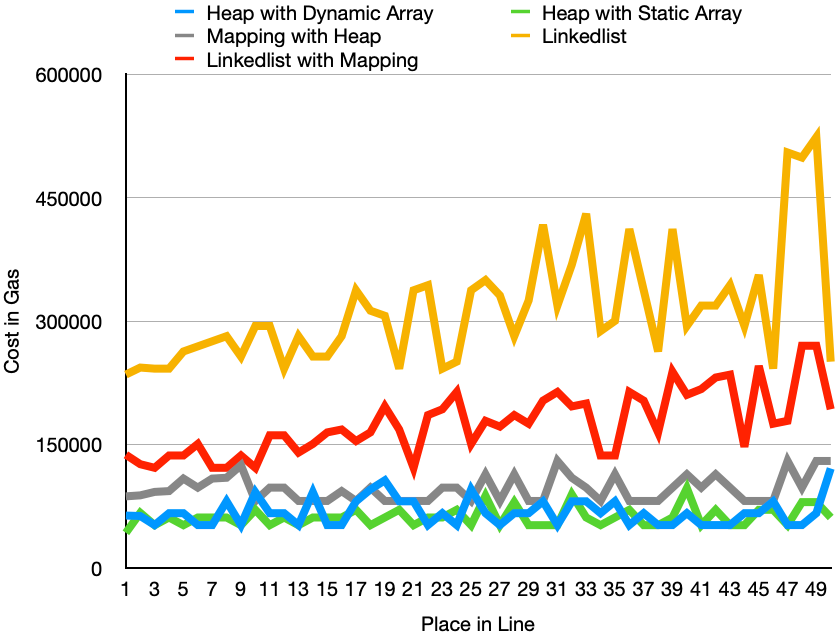
\includegraphics[width=1\textwidth]{fig/average_uints_insertion.png}
\caption{\footnotesize{}  \label{fig:average_uints_insertion}}
\end{figure}

% = = = = = = = = = = = = = = = = = = = = = = = = = = = = = = = = = = = = = = = =  %

Then, we call the \texttt{Dequeue()} function which iteratively removes the maximum value of the priority queue (until the data structure is empty). The computational costs for dequeuing 50 unsigned integers in each priority queue are outlined in Table~\ref{tab:PQ_UnitTests}. The tests are performed using the current Ethereum gas metrics (block gas limit $=$11,741,495 and 1 gas $=$ 56 gwei)~\footnote{https://ethstats.net/}. The second column of the table shows the net gas consumption (the gasUsed value derived from transaction receipts) for removing 50 integers from each priority queues.  

At the time of this writing, Ethereum transaction receipts only contain the net gas consumption and not the total gas consumption ( total gas consumption is defined as $gas refunded + gasUsed$ ) and we cannot find out the value of the EVM's refund counter from inside the EVM.

So in order to account for refunds inside each priority queue smart contract, we can calculate them manually; first we figure out exactly how much storage is being cleared when dequeuing  the max integers and then we could multiply the number of storage slots cleared by 15,000 (see the last column of Table~\ref{tab:PQ_UnitTests}).

Another way to know the amount of refund in each priority queue is to use the \texttt{estimateGas API} which provides a rough idea about the total amount of gas that is required for a transaction to go through. The \texttt{web3.eth.estimateGas} pretends the transaction is included in the block and its functions (with the parameters passed) will be executed on the Ethereum blockchain. Doing so, it provides us an estimate of how much gas is needed to be sent with the transaction. The second and third columns of Table~\ref{tab:PQ_UnitTests}) show the total amount of gas required for dequeuing 50 integers from each priority queue (provided by estimateGas) and the amount of gas refund ($Total Gas Consumption - gasUsed$) respectively.

Note that in order to urge miners to process smart contract with refunds, the accumulated gas refund can never exceed half the gas used up during computation~\cite{wood2014ethereum}. So at the end of a successful transaction, the amount of gas in the refund counter (capped at half the net gas used) is returned to the caller. For example, the amount of gas that has been used when dequeuing 50 integers from the linkedlist with mapping data structure is 731,514 and since $3,000,000 > 731,514/2$, the amount of refund returned to the caller is $731,514/2 = 365,757$.

% = = = = = = = = = = = =Uint testing the PQs Table = = = = = = = = = = = = =  %

\begin{table}[]
\centering
\begin{tabular}{|c|c|c|c|c|}
\hline

\textbf{\thead{Priority Queue}}    & \textbf{\thead{Net Cost\\in Gas}}      & \textbf{\thead{Total Cost\\in Gas\\(from estimateGas)}}      & \textbf{\thead{Gas Refund \\(from \texttt{estimateGas})}}    & \textbf{\thead{Gas Refund \\(Manually Calculated)}} \\ \hline

% = = = = = = = = = = = = = = = = = = = = = = = = = = = = = = = = = = = = = = = = = = = = = = = = = = = = = = = = = = = = = = = = = = = = = = %
	\textbf{\thead{Heap with \\ Dynamic Array}}         				& 2,547,031               & 3,312,378		& 765,347             & 750,000                       \\ \hline
% = = = = = = = = = = = = = = = = = = = = = = = = = = = = = = = = = = = = = = = = = = = = = = = = = = = = = = = = = = = = = = = = = = = = = = %
	\textbf{\thead{Heap with \\ Static Array}}           				& 1,324,856                & 2,090,182     	& 765,326             & 750,000                      \\ \hline
% = = = = = = = = = = = = = = = = = = = = = = = = = = = = = = = = = = = = = = = = = = = = = = = = = = = = = = = = = = = = = = = = = = = = = = %
	\textbf{\thead{Mapping with \\ keys stored \\ in Heap}} 		& 2,863,239                & 4,378,584       	& 1,515,345           & 1,500,000                     \\ \hline
% = = = = = = = = = = = = = = = = = = = = = = = = = = = = = = = = = = = = = = = = = = = = = = = = = = = = = = = = = = = = = = = = = = = = = = %
	\textbf{Linkedlist}                       							& 557,085               	& 1,772,085      	& 1,215,000           & 1,200,000                      \\ \hline
% = = = = = = = = = = = = = = = = = = = = = = = = = = = = = = = = = = = = = = = = = = = = = = = = = = = = = = = = = = = = = = = = = = = = = = %
	\textbf{\thead{Linkedlist with \\ Mapping}}          				& 731,514              	& 3,731,514       	& 3,000,000     	  &  3,765,000                       \\ \hline
% = = = = = = = = = = = = = = = = = = = = = = = = = = = = = = = = = = = = = = = = = = = = = = = = = = = = = = = = = = = = = = = = = = = = = = %

\end{tabular}
\caption{\footnotesize{}
\label{tab:PQ_UnitTests}}
\end{table}
% = = = = = = = = = = = = = = = = = = = = = = = = = = = = = = = = = = = = =  %



%============= Experiments =================== %
\section{Experiments}

Our application was developed in Solidity using the Truffle development framework and deployed on Ganache-CLI. We used Javascript for testing by leveraging the Mocha testing framework. Followings outline the results of different tests we performed.

%============= Test 1 (17_Worst_Case_Matching_test.js) Tables=================== %

 \subsection{Experiments on the \texttt{Match()} Function}

We executed the same test on the the five different versions of the CallMarket we implemented using five priority queues to examine the cost of the \texttt{Match()} function as well as the maximum pairs of bid and ask orders it can handle in each case. The \texttt{Match()} function's computational cost and the maximum number of orders it can execute in each case (before running out of gas) are outlined in Table~\ref{tab:worst_case_matching}. Note that this is a \textit{worst case matching} test where all bids and asks are submitted as marketable limit orders with specified prices that would be filled undoubtedly, performed using the current Ethereum gas metrics (block gas limit $=$11,741,495 and 1 gas $=$ 56 gwei)~\footnote{https://ethstats.net/}. The last column of Table~\ref{tab:worst_case_matching} shows the gas cost of matching 1000 pairs of bids and asks for each priority queue for which we set the block gas limit to the maximum of  $2^{53}$ (the Javascript's max safe integer).


%======= estimateGas() function = gasUsed + gasRefund =======%

% Heap with Dynamic Array: match.estimateGas() = 7204994 => gasRefund = 7204994 - 3274994 = 3930000
% Heap with Static Array: match.estimateGas() = 7337527 => gasRefund = 7337527 - 3107527 = 4230000
% Mapping with keys stored in Heap: match.estimateGas() = 6644803 => gasRefund = 6644803 - 5414803 = 1230000
% Linkedlist: match.estimateGas() = 7629847 => gasRefund = 7629847 -  3279847 = 4350000
% Linkedlist with Mapping: match.estimateGas() = 7227717 => gasRefund = 7227717 -  3297717 = 3930000

%===============================================%


% = = = = = = = = = = = =Worst_Case_Matching Table = = = = = = = = = = = = =  %

\begin{table}[]
\centering
\begin{tabular}{|c|c|c|c|}
\hline

\textbf{\thead{Priority Queue}}    & \textbf{\thead{Maximum Number \\ of \\ Matched Orders}}      & \textbf{\thead{Net Cost\\in Gas}}          & \textbf{\thead{Net Cost in Gas\\ for \\ 1000 Pairs \\ of Orders}} \\ \hline

% = = = = = = = = = = = = = = = = = = = = = = = = = = = = = = = = = = = = = = = = = = = = = = = = = = = = = = = = = = = = = = = = = = = = = = %
	\textbf{\thead{Heap with \\ Dynamic Array}}         				& 26 pairs                & 3,274,994                   	& 457,326,935                      \\ \hline
% = = = = = = = = = = = = = = = = = = = = = = = = = = = = = = = = = = = = = = = = = = = = = = = = = = = = = = = = = = = = = = = = = = = = = = %
	\textbf{\thead{Heap with \\ Static Array}}           				& 28 pairs                & 3,107,527                  	& 333,656,805                       \\ \hline
% = = = = = = = = = = = = = = = = = = = = = = = = = = = = = = = = = = = = = = = = = = = = = = = = = = = = = = = = = = = = = = = = = = = = = = %
	\textbf{\thead{Mapping with \\ keys stored \\ in Heap}} 		& 40 pairs                & 5,414,803                     & 319,481,722                       \\ \hline
% = = = = = = = = = = = = = = = = = = = = = = = = = = = = = = = = = = = = = = = = = = = = = = = = = = = = = = = = = = = = = = = = = = = = = = %
	\textbf{Linkedlist}                       							& 90 pairs                & 3,279,847                      & 35,823,601                        	\\ \hline
% = = = = = = = = = = = = = = = = = = = = = = = = = = = = = = = = = = = = = = = = = = = = = = = = = = = = = = = = = = = = = = = = = = = = = = %
	\textbf{\thead{Linkedlist with \\ Mapping}}          				& 130 pairs              & 3,297,717                       & 25,095,370                        \\ \hline
% = = = = = = = = = = = = = = = = = = = = = = = = = = = = = = = = = = = = = = = = = = = = = = = = = = = = = = = = = = = = = = = = = = = = = = %

\end{tabular}
\caption{\footnotesize{}
\label{tab:worst_case_matching}}
\end{table}



%%============= Test 3 (17_Worst_Case_Submission_test.js) Figures==================== %
%
% \subsection{Experiments on \texttt{Submit Order()} Functions}
%
%We executed another set of tests on the the five different versions of the CallMarket in which we sent 200 \texttt{SubmitBid} to the CallMarket to simulate two hundred of traders participating in the market. These tests were performed in two levels (i) worst case and (ii) average case submissions. 
%%the data structure used for bids and asks is the same and hence the submission plots for 200 submitbids and 200 submitasks. Do we have to mention that here?
%
%% = = = = = = = = = = = =Worst_Case_Submission = = = = = = = = = = = = =  %
%
%\subsubsection{Worst Case Order Submission}
%
%Here each \texttt{SubmitBid()} transaction has a price that is smallest or second-smallest of the transactions after it. Doing so, we ensure all the orders move every time a new order is sent to the market. Figure~\ref{fig:worst_case_submission} shows the gas cost variations for submitting 200 orders in five versions of the CallMarket. The x-axis is the place in line (\eg the 10th person to submit the order) and the and y-axis is the gas cost for sending that transaction.
%
%%And conversely each \texttt{SubmitAsk()} transaction has a price that is biggest or second-biggest of the transactions after it
%
%% = = = = = = = = = = = =Worst_Case_Submission Figure = = = = = = = = = = = = =  %
%
%\begin{figure}[htb!p]
%\centering
%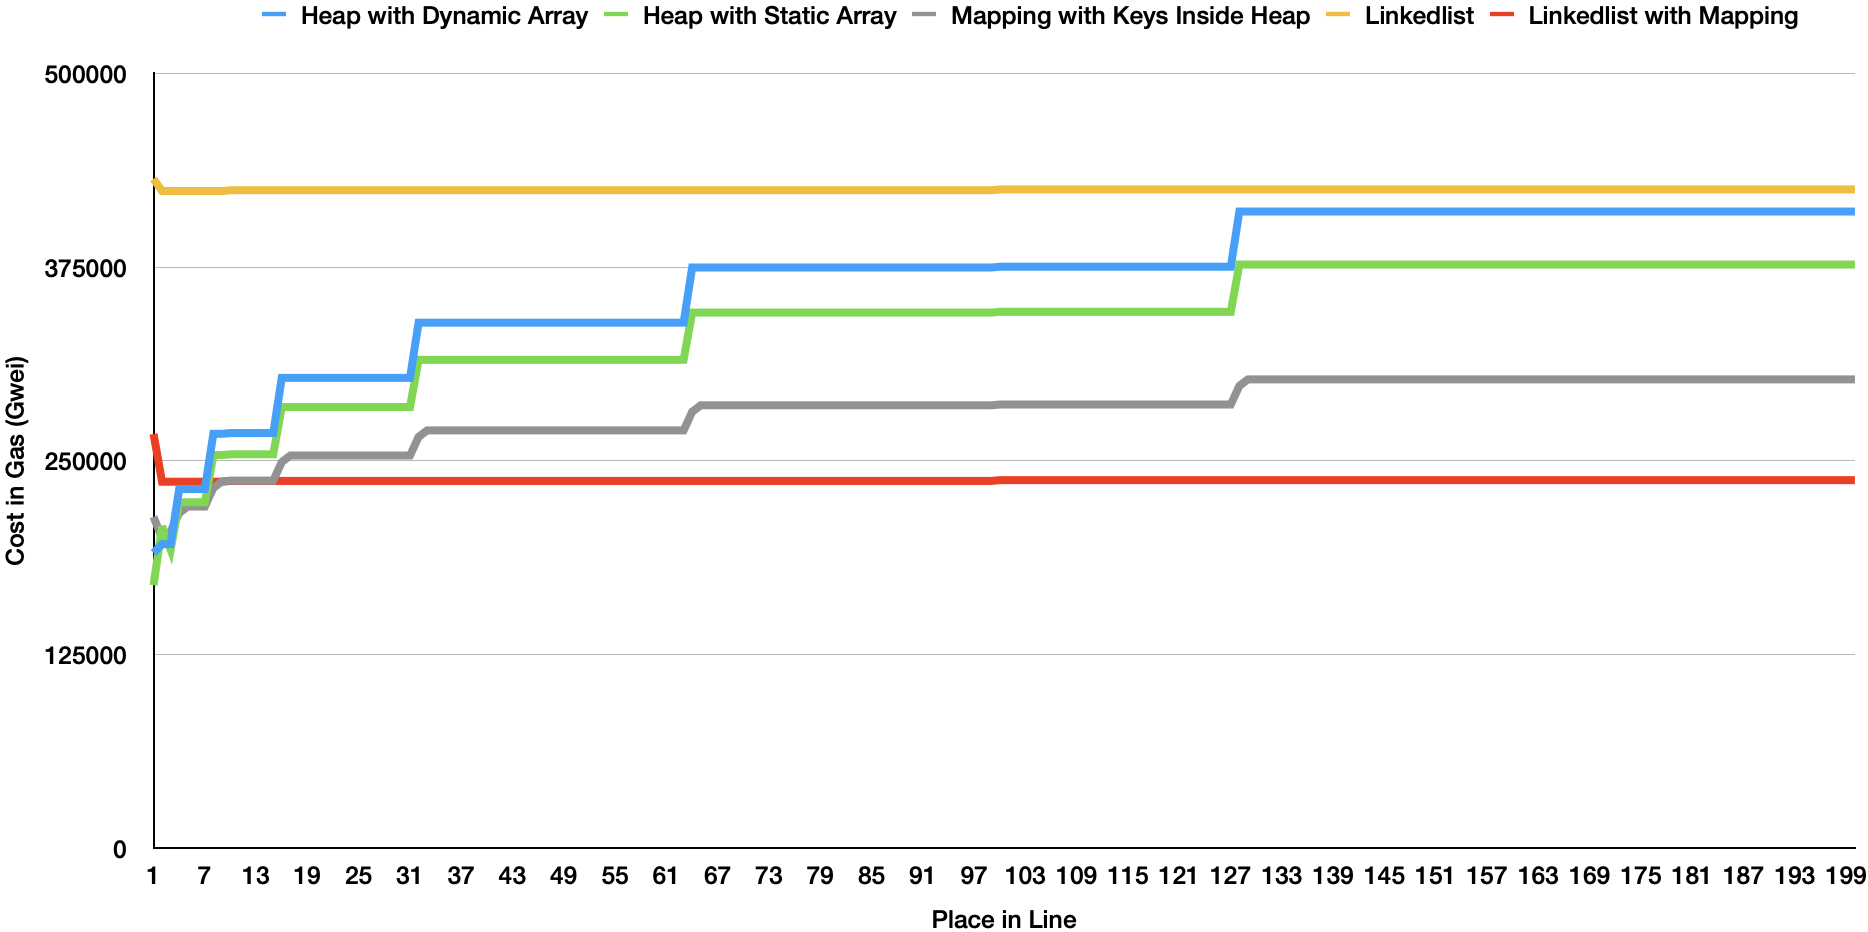
\includegraphics[width=1\textwidth]{fig/worst_case_submission_3.png}
%\caption{\footnotesize{}  \label{fig:worst_case_submission}}
%\end{figure}
%
%% = = = = = = = = = = = = = = = = = = = = = = = = = = = = = = = = = = = = = = = =  %
%
%
%% = = = = = = = = = = = =Average_Case_Submission = = = = = = = = = = = = =  %
%
%\subsubsection{Average Case Order Submission}
%
%Here we test the five versions of the CallMarket when 200 bid orders are entered in random ordering. To do so, we use JavaScript \texttt{Math.random()} function to generate pseudo-random integers between 1 and 100. Figure~\ref{fig:average_case_submission} shows the gas cost variations for submitting 200 orders in five versions of the CallMarket. Again the x-axis is the place in line (\eg the10th person to submit the order) and the and y-axis is the gas cost for submitting that transaction. 
%
%% = = = = = = = = = = = =Average_Case_Submission Figure = = = = = = = = = = = = =  %
%
%\begin{figure}[htb!p]
%\centering
%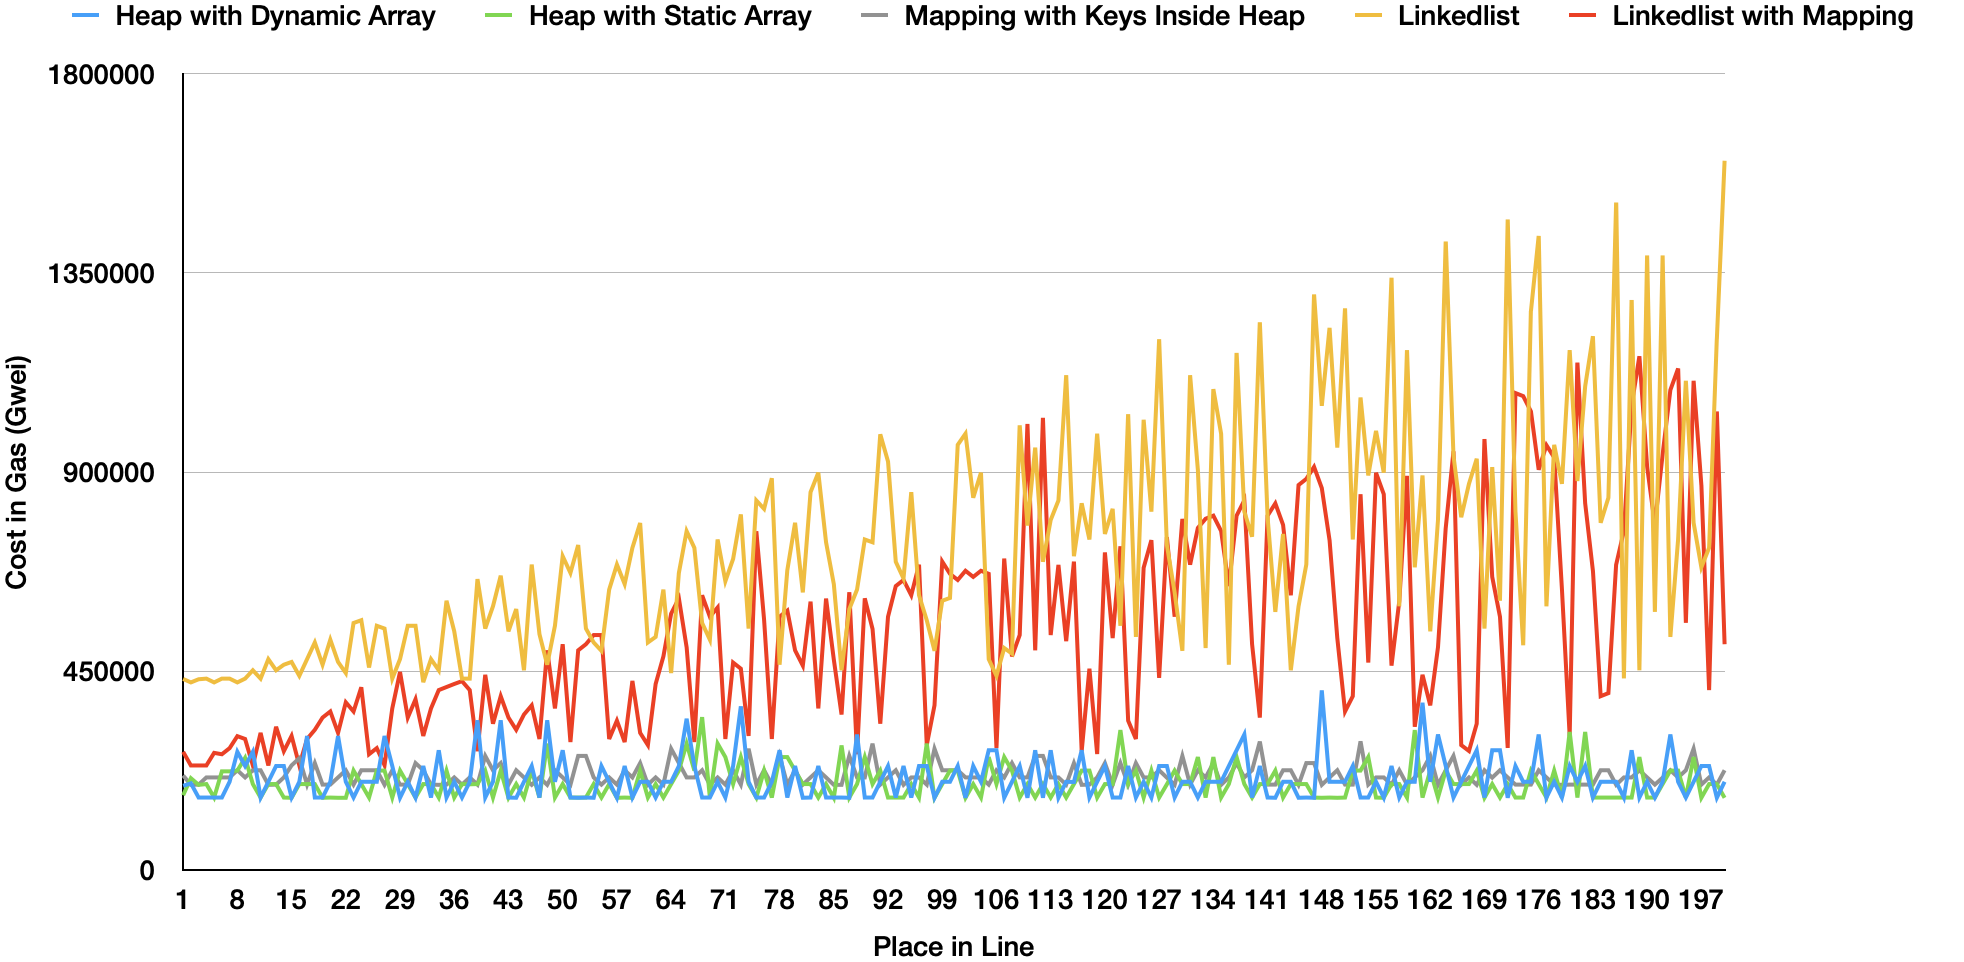
\includegraphics[width=1\textwidth]{fig/average_case_submission_3.png}
%\caption{\footnotesize{}  \label{fig:average_case_submission}}
%\end{figure}
%
%% = = = = = = = = = = = = = = = = = = = = = = = = = = = = = = = = = = = = = = = =  %














%======================================== %

% = = = = = = = = = = = = = = = = = = = = = = = = = = = = = = = = = = = = = = = = = =

\section{Concluding Remarks}


 
%\subsubsection*{Acknowledgements.} J. Clark thanks ...

































